\documentclass[t]{beamer}
\usetheme[progressbar=frametitle]{metropolis}
\usepackage{appendixnumberbeamer}

\usepackage{booktabs}
\usepackage[scale=2]{ccicons}

\usepackage{graphics,graphicx,amssymb,amsmath,pgf,comment,hyperref}
%\usepackage[xcolor=pst]{pstricks}
\usepackage{array}
\usepackage{pgfshade}
\usepackage[round]{natbib}
\usepackage[absolute,overlay]{textpos}
\usepackage{pifont}
\usepackage{dcolumn}
\usepackage{textpos}
\usepackage{color}					
\usepackage{xcolor,colortbl}
\usepackage{tikz}
\usepackage{bbm}
\usepackage{curves}
\usepackage{mathtools}
\usetikzlibrary{snakes,arrows,positioning}
\def\augie{\fontencoding{T1}\fontfamily{augie}\selectfont}

\usepackage{pgfplots}
\usepgfplotslibrary{dateplot}

\usepackage{xspace}
\newcommand{\themename}{\textbf{\textsc{metropolis}}\xspace}

\setbeamertemplate{caption}{\raggedright\insertcaption\par}
\usetikzlibrary{calc,decorations.pathmorphing,patterns}
\pgfdeclaredecoration{penciline}{initial}{
    \state{initial}[width=+\pgfdecoratedinputsegmentremainingdistance,
    auto corner on length=1mm,]{
        \pgfpathcurveto%
        {% From
            \pgfqpoint{\pgfdecoratedinputsegmentremainingdistance}
                      {\pgfdecorationsegmentamplitude}
        }
        {%  Control 1
        \pgfmathrand
        \pgfpointadd{\pgfqpoint{\pgfdecoratedinputsegmentremainingdistance}{0pt}}
                    {\pgfqpoint{-\pgfdecorationsegmentaspect
                     \pgfdecoratedinputsegmentremainingdistance}%
                               {\pgfmathresult\pgfdecorationsegmentamplitude}
                    }
        }
        {%TO
        \pgfpointadd{\pgfpointdecoratedinputsegmentlast}{\pgfpoint{1pt}{1pt}}
        }
    }
    \state{final}{}
}


\title{Physician Behaviors and Hospital Influence}
\date{Emory University}
\author{Haizhen Lin \& \textbf{Ian McCarthy} \& Michael Richards}
\institute{October 18, 2018}

\begin{document}

\maketitle

\section{Background}

\begin{frame}{How are hospitals and physicians related?}
    \only<1>{
        \begin{enumerate}
            \item ``Traditional'' private practice with admitting privileges
            \item Administrative support with or without admitting restrictions
            \item Practice owned by hospital or hospital system
        \end{enumerate}
    }
    \only<2>{
        \begin{figure}
            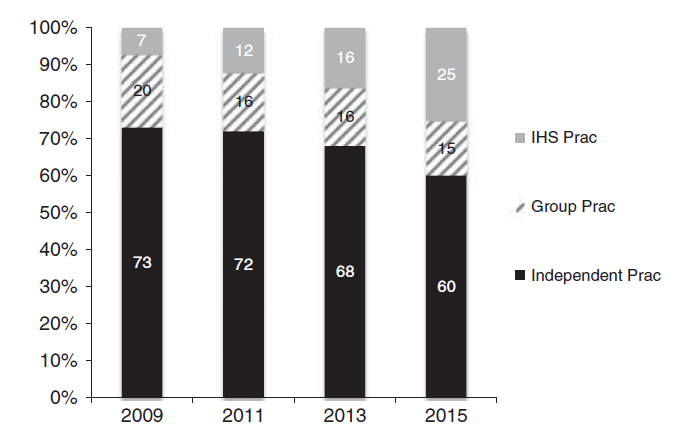
\includegraphics[height=2.4in,keepaspectratio]{Richardsetal.png}
            \caption{Richards \textit{et al.}, Medical Care, 2016}
        \end{figure}
    }
    \only<3>{
        \begin{figure}
            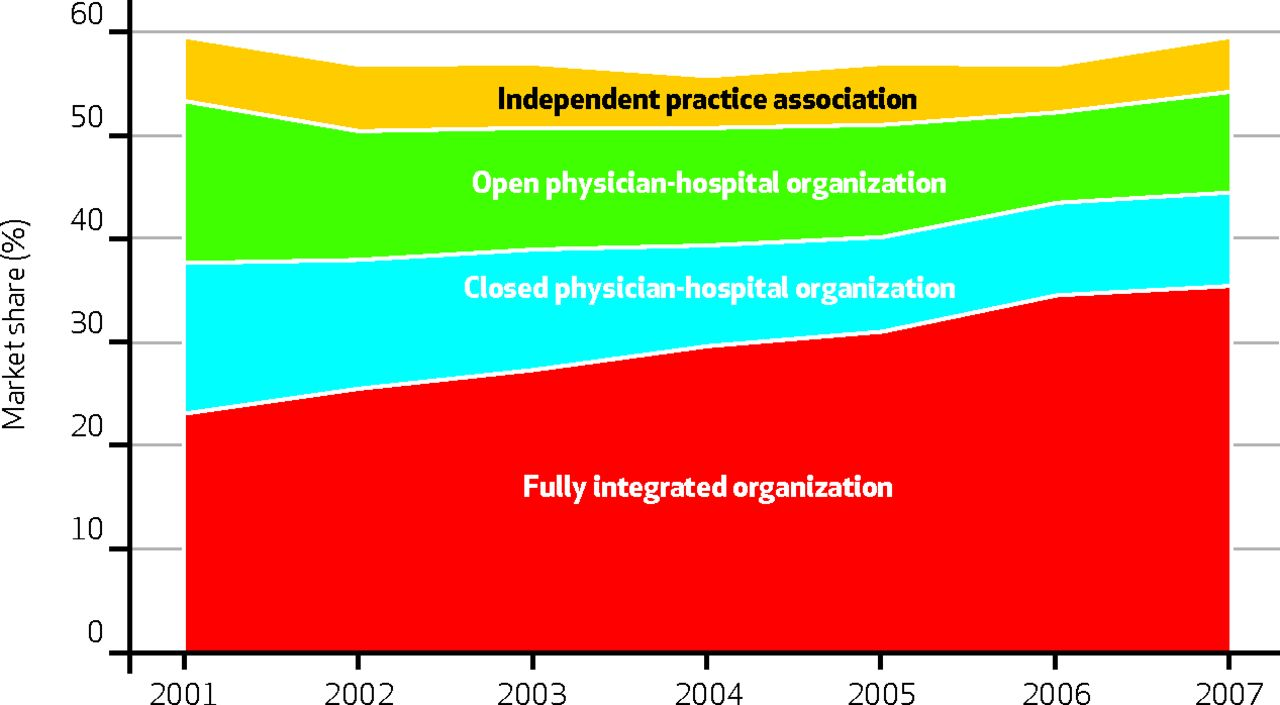
\includegraphics[height=2.3in,keepaspectratio]{Bakeretal.jpg}
            \caption{Baker, Bundorf, and Kessler, Health Affairs, 2014}
        \end{figure}
    }
\end{frame}

\begin{frame}{Why would a hospital integrate?}
    \only<1>{
        \metroset{block=fill}
        \begin{block}{Direct Revenue}
            \begin{itemize}
                \item Increase bargaining position
                \item Exploit payment differentials
            \end{itemize}
        \end{block}
    }

    \only<2>{
        \metroset{block=fill}
        \begin{block}{Indirect Revenue}
            \begin{itemize}
                \item Hospital Readmission Reduction Program
                \item Hospital Value Based Purchasing Program
                \item Accountable Care Organizations and Bundled Payments
                \item Product Bundling
            \end{itemize}
        \end{block}
    }

    \only<3>{
        \metroset{block=fill}
        \begin{block}{Cost reduction}
            \begin{itemize}
                \item Remove inefficiencies from fragmented care
                \item Improve quality via ``team-based'' care
                \item Faster time to discharge
                \item Streamline devices
            \end{itemize}
        \end{block}
    }
\end{frame}

\begin{frame}{Why would a physician practice integrate?}
    \only<1>{
        \metroset{block=fill}
        \begin{block}{Financial security}
            \begin{itemize}
                \item Salaried arrangement
                \item Potential volume incentives
            \end{itemize}
        \end{block}
    }

    \only<2>{
        \metroset{block=fill}
        \begin{block}{Reduce administrative burden}
            \begin{itemize}
                \item Billing and insurance approvals
                \item Electronic Health Records
                \item Data collection/reporting
            \end{itemize}
        \end{block}
    }
\end{frame}

\begin{frame}{Takeaway}
    \begin{enumerate}
        \item Incentives for the hospitals to influence physician behaviors
        \item Willingness by physicians to allow influence
    \end{enumerate}
\end{frame}


\section{Theoretical Framework}
\begin{frame}{Measuring Physician Agency}
    Observed care at time $t$ is
    \begin{equation*}
        y_{ijk} = \arg \max_{y}  \theta_{u} \tilde{u} \left(y; \Gamma_{j}, \kappa_{i} \right) + \theta_{\pi} \pi \left(y; \Gamma_{k}, \Gamma_{j} \right),
    \end{equation*}
    where $\tilde{u}$ is additively separable in $i$ and $(j,k)$ and where maximizing levels of $y$ for $\tilde{u}$ and $\pi$ are linear in $y$
\end{frame}

\begin{frame}{Measuring Physician Agency}
    \begin{equation*}
        y_{ijk} = \alpha_{i} + x_{i}\beta + \Gamma_{jk} + \epsilon_{ijk},
    \end{equation*}
    \begin{itemize}
        \item $\alpha_{i}$, unobserved patient characteristics
        \item $x_{i}$, observed patient characteristics
        \item $\Gamma_{jk}$, a function of observed and unobserved physician and hospital characteristics
    \end{itemize}
\end{frame}

\begin{frame}{Variation in Physician Agency}
    What characteristics of the hospital, physician, and physician practice tend to drive variation in care, conditional on patient preferences?
    \begin{equation*}
        \Gamma_{jkt} = \gamma_{j} + \gamma_{k} + \tau_{t} + z_{jkt}\delta + \eta_{jkt},
    \end{equation*}
    \begin{itemize}
        \item $\gamma_{j}$, unobserved and time-invariant physician characteristics
        \item $\gamma_{k}$, unobserved and time-invariant hospital characteristics
        \item $\tau_{t}$, unobserved year factors affecting all physicians and hospitals
        \item $z_{jkt}$, observed and time-varying physician and hospital characteristics
    \end{itemize}
\end{frame}


\section{Data}
\begin{frame}{Data Sources}
    \begin{itemize}
        \item<1-> CMS: 100\% inpatient Medicare claims data (2008-2015)
        \item<2-> SK\&A: Hospital ownership of physician practices
        \item<3-> AHA, HCRIS, POS: Hospital characteristics
        \item<4-> ACS: County-level demographics, education, income, and employment
    \end{itemize}
\end{frame}

\begin{frame}{Sample Construction}
    \begin{itemize}
        \item<1-> Planned inpatient operations with observed NPI for the operating physician, defined as elective admissions initiated by a physician, clinic, or HMO referral
        \item<2-> Drop physicians operating in hospitals more than 120 miles from primary office or outside of contiguous U.S.
        \item<3-> Drop physicians with NPIs not matched in the SK\&A data
        \item<4-> Drop lowest/highest 1\% of inpatient charges and patients $<$ 65 years old
    \end{itemize}
  \uncover<5->{ $\Longrightarrow$ 518,398 unique observations at the physician/hospital/year \\
   $\Longrightarrow$ 7.5mm inpatient stays (47\% of total)}
\end{frame}



\section{Estimation of Match Values}
\begin{frame}{Specification}
    \begin{equation*}
        y_{ijk} = \alpha_{i} + x_{i}\beta + \Gamma_{jk} + \epsilon_{ijk},
    \end{equation*}
\end{frame}

\begin{frame}{Outcomes}
    \begin{equation*}
        \textcolor{red}{y_{ijk}} = \alpha_{i} + x_{i}\beta + \Gamma_{jk} + \epsilon_{ijk},
    \end{equation*}

    \begin{itemize}
        \item Inpatient charges
        \item Length of stay
        \item 30/60/90-day mortality
    \end{itemize}
\end{frame}


\begin{frame}{Independent Variables}
    \begin{equation*}
        y_{ijk} = \textcolor{red}{\alpha_{i}} + x_{i}\beta + \Gamma_{jk} + \epsilon_{ijk},
    \end{equation*}

    \begin{itemize}
        \item Quartiles of total Medicare payments and inpatient claims
        \item Covers 2008 through 2015 period
        \item Beneficiary-specific measure of ``utilization''
    \end{itemize}
\end{frame}

\begin{frame}{Independent Variables}
    \begin{equation*}
        y_{ijk} = \alpha_{i} + \textcolor{red}{x_{i}}\beta + \Gamma_{jk} + \epsilon_{ijk},
    \end{equation*}

    \begin{itemize}
        \item Age
        \item Gender
        \item Race
        \item Dummies for first 5 ICD diagnosis codes (18 diagnosis groups per variable plus missing group)
    \end{itemize}
\end{frame}


\begin{frame}{Within-physician Variation in Charges}
    \begin{figure}
        \centering
        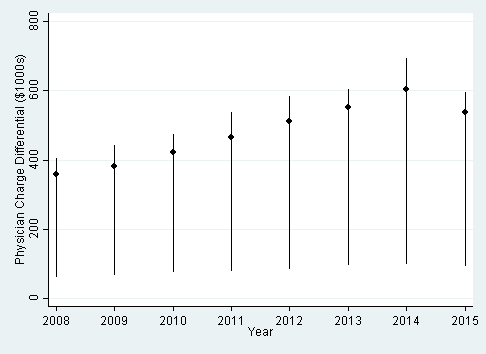
\includegraphics[height=2.5in,width=5in,keepaspectratio]{PhySave_Graph}
    \end{figure}
\end{frame}

\begin{frame}{Within-physician Variation in LOS}
    \begin{figure}
        \centering
        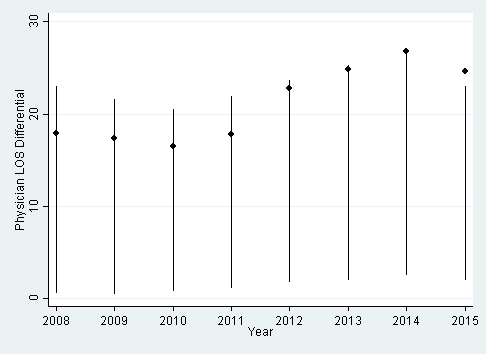
\includegraphics[height=2.5in,width=5in,keepaspectratio]{PhyLOS_Graph} \\
    \end{figure}
\end{frame}

\begin{frame}{Within-hospital Variation in Charges}
    \begin{figure}
        \centering
        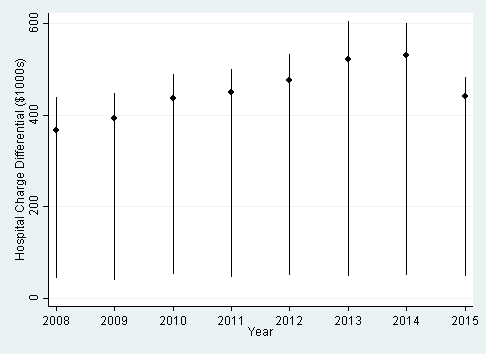
\includegraphics[height=2.5in,width=5in,keepaspectratio]{HospSave_Graph_DRG}
    \end{figure}
\end{frame}

\begin{frame}{Within-hospital Variation in LOS}
    \begin{figure}
        \centering
        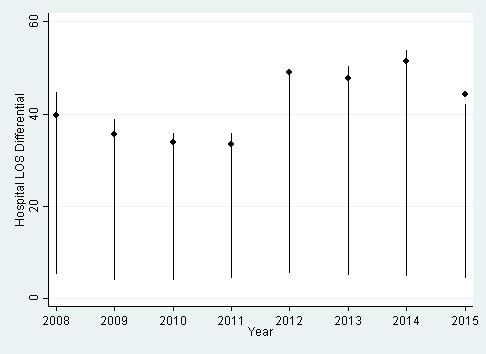
\includegraphics[height=2.5in,width=5in,keepaspectratio]{HospLOS_Graph_DRG}
    \end{figure}
\end{frame}


\section{Estimation of Institutional Influence}
\begin{frame}{Specification}
    \begin{equation*}
        \hat{\Gamma}_{jkt} = \gamma_{j} + \gamma_{k} + \tau_{t} + z_{jkt}\delta + \eta_{jkt},
    \end{equation*}
\end{frame}

\begin{frame}{Outcomes: Hospital Share and Operations}
    \begin{equation*}
        \textcolor{red}{\hat{\Gamma}_{jkt}} = \gamma_{j} + \gamma_{k} + \tau_{t} + z_{jkt}\delta + \eta_{jkt},
    \end{equation*}

    \begin{table}[htb!]
    \centering
    \footnotesize
    \centerline{
    \begin{tabular}{l|rrrrr|r}
        & 2008  & 2012 & 2013 & 2014 & 2015 & Overall \\
        \hline
Hospital Share&       0.687         &       0.713         &       0.719         &       0.726         &       0.753         &       0.712         \\
              &     (0.366)         &     (0.357)         &     (0.356)         &     (0.353)         &     (0.339)         &     (0.358)         \onslide<2->{\\
Operations    &       18.55         &       18.21         &       18.61         &       18.82         &       20.23         &       18.58         \\
              &     (26.03)         &     (26.02)         &     (26.94)         &     (27.32)         &     (28.87)         &     (26.46)         }\\
    \end{tabular}}
    \end{table}

\end{frame}

\begin{frame}{Outcomes: Charges and Length of Stay}
    \begin{equation*}
        \textcolor{red}{\hat{\Gamma}_{jkt}} = \gamma_{j} + \gamma_{k} + \tau_{t} + z_{jkt}\delta + \eta_{jkt},
    \end{equation*}

    \begin{table}[htb!]
    \centering
    \footnotesize
    \centerline{
    \begin{tabular}{l|rrrrr|r}
        & 2008  & 2012 & 2013 & 2014 & 2015 & Overall \\
        \hline
Hospital Charge  &     41,829         &     56,920         &     61,780         &     66,497         &     69,965         &     54,549         \\
                 &   (27,807)         &   (37,505)         &   (40,228)         &   (43,196)         &   (46,204)         &   (37,579)         \onslide<2->{\\
Length of Stay   &       5.984         &       6.021         &       6.002         &       6.062         &       6.031         &       5.960         \\
                 &     (2.427)         &     (2.493)         &     (2.494)         &     (2.513)         &     (2.613)         &     (2.449)}         \\
    \end{tabular}}
    \end{table}

\end{frame}

\begin{frame}{Outcomes: Mortality}
    \begin{equation*}
        \textcolor{red}{\hat{\Gamma}_{jkt}} = \gamma_{j} + \gamma_{k} + \tau_{t} + z_{jkt}\delta + \eta_{jkt},
    \end{equation*}

    \begin{table}[htb!]
    \centering
    \footnotesize
    \centerline{
    \begin{tabular}{l|rrrrr|r}
        & 2008  & 2012 & 2013 & 2014 & 2015 & Overall \\
        \hline
90-day Mortality &      0.0628         &      0.0604         &      0.0586         &      0.0575         &      0.0569         &      0.0600         \\
                 &     (0.147)         &     (0.144)         &     (0.143)         &     (0.140)         &     (0.145)         &     (0.145)         \onslide<2->{\\
60-day Mortality &      0.0521         &      0.0497         &      0.0485         &      0.0475         &      0.0461         &      0.0495         \\
                 &     (0.133)         &     (0.130)         &     (0.130)         &     (0.127)         &     (0.131)         &     (0.131)         \onslide<3->{\\
30-day Mortality &      0.0375         &      0.0354         &      0.0349         &      0.0340         &      0.0318         &      0.0353         \\
                 &     (0.113)         &     (0.109)         &     (0.110)         &     (0.107)         &     (0.108)         &     (0.110)         }}\\
    \end{tabular}}
    \end{table}
\end{frame}


\begin{frame}{Independent Variables}
    \begin{equation*}
        \hat{\Gamma}_{jkt} = \gamma_{j} + \gamma_{k} + \tau_{t} + \textcolor{red}{z_{jkt}}\delta + \eta_{jkt},
    \end{equation*}

    \begin{table}[htb!]
    \centering
    \footnotesize
    \centerline{
    \begin{tabular}{l|rrrrr|r}
        & 2008  & 2012 & 2013 & 2014 & 2015 & Overall \\
        \hline
Integrated       &       0.130         &       0.206         &       0.233         &       0.255         &       0.332         &       0.196         \\
                 &     (0.336)         &     (0.404)         &     (0.422)         &     (0.436)         &     (0.471)         &     (0.397)         \onslide<2->{\\
Physician FTE       &       24.23         &       28.59         &       31.14         &       31.74         &       33.13         &       28.43         \\
                    &     (99.28)         &     (109.8)         &     (120.5)         &     (120.0)         &     (119.5)         &     (110.9)         \onslide<3->{\\
Resident FTE        &       25.77         &       28.45         &       29.13         &       30.69         &       30.97         &       28.08         \\
                    &     (108.2)         &     (120.4)         &     (121.4)         &     (125.9)         &     (127.8)         &     (117.8)         \onslide<4->{\\
Nurse FTE           &       340.8         &       365.7         &       369.1         &       384.9         &       402.7         &       364.8         \\
                    &     (446.8)         &     (487.8)         &     (494.8)         &     (519.1)         &     (550.7)         &     (487.3)         \onslide<5->{\\
Other FTE           &       749.9         &       763.0         &       761.8         &       776.4         &       806.0         &       762.8         \\
                    &     (975.5)         &    (1032.4)         &    (1076.2)         &    (1101.5)         &    (1157.2)         &    (1037.4)         \onslide<6->{\\
Beds (100s)         &       1.980         &       1.967         &       1.958         &       1.982         &       2.009         &       1.976         \\
                    &     (2.160)         &     (2.142)         &     (2.137)         &     (2.172)         &     (2.235)         &     (2.154)         }}}}}\\
    \end{tabular}}
    \end{table}

\end{frame}

\begin{frame}{Independent Variables}
    \begin{equation*}
        \hat{\Gamma}_{jkt} = \gamma_{j} + \gamma_{k} + \tau_{t} + \textcolor{red}{z_{jkt}}\delta + \eta_{jkt},
    \end{equation*}

    \begin{table}[htb!]
    \centering
    \footnotesize
    \centerline{
    \begin{tabular}{l|rrrrr|r}
        & 2008  & 2012 & 2013 & 2014 & 2015 & Overall \\
        \hline
Practice Size&       13.73         &       17.31         &       17.31         &       17.82         &       18.41         &       16.10         \\
             &     (32.10)         &     (30.70)         &     (29.28)         &     (28.46)         &     (28.02)         &     (30.05)         \onslide<2->{\\
Experience   &       22.55         &       23.00         &       23.94         &       23.65         &       24.77         &       23.17         \\
             &     (6.496)         &     (6.703)         &     (6.950)         &     (6.902)         &     (6.989)         &     (6.746)         \onslide<3->{\\
\% Multi-Specialty &       0.249         &       0.248         &       0.266         &       0.284         &       0.344         &       0.264         \\
\% with Surgery &       0.452         &       0.501         &       0.507         &       0.508         &       0.454         &       0.480         }}\\
    \end{tabular}}
    \end{table}

\end{frame}

\begin{frame}{Initial Results}
    \begin{table}[htb!]
    \centering
    \footnotesize
    \centerline{
    \begin{tabular}{l|rrr}
        & Vert. Int.      & Practice Size & Beds \\
        \hline
        \multicolumn{3}{l}{Mean Outcomes} \\
        \hline
        Share           &       0.068*** &       0.000*   &       0.003*** \\
                        &     (0.003)    &     (0.000)    &     (0.001)    \\
        Operations      &       1.166*** &       0.013*** &       0.061    \\
                        &     (0.165)    &     (0.003)    &     (0.066)    \\
        Charge          &     978.334*** &      23.713*** &     154.701    \\
                        &   (215.302)    &     (4.234)    &    (95.896)    \\
        LOS             &      -0.001    &       0.001*** &       0.020**  \\
                        &     (0.017)    &     (0.000)    &     (0.008)    \\
    \end{tabular}}
    \end{table}
\end{frame}

\begin{frame}{Initial Results}
    \begin{table}[htb!]
    \centering
    \footnotesize
    \centerline{
    \begin{tabular}{l|rrr}
        & Vert. Int.      & Practice Size & Beds \\
        \hline
        \multicolumn{3}{l}{$\Gamma_{jkt}$} \\
        \hline
        Charge          &     824.251*** &      22.890*** &     163.798*   \\
                        &   (187.598)    &     (3.669)    &    (87.130)    \\
        LOS             &      -0.007    &       0.002*** &       0.012    \\
                        &     (0.017)    &     (0.000)    &     (0.008)    \onslide<2->{\\
        \hline
        \multicolumn{3}{l}{$\Gamma_{jkt}$ with quality} \\
        \hline
        Charge          &     808.072*** &      22.649*** &     160.556*   \\
                        &   (187.311)    &     (3.660)    &    (86.871)    \\
        LOS             &      -0.008    &       0.002*** &       0.012    \\
                        &     (0.017)    &     (0.000)    &     (0.008)    }\\
    \end{tabular}}
    \end{table}
\end{frame}



\begin{frame}{Event Study}
    \begin{figure}
        \centering
        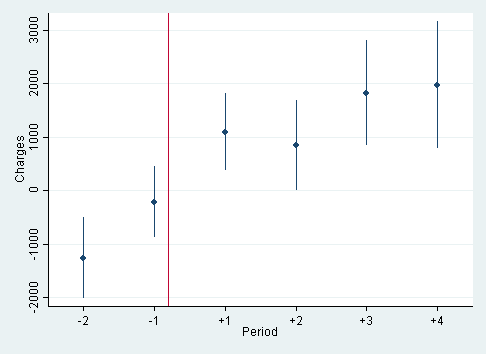
\includegraphics[height=2.5in,width=5in,keepaspectratio]{EventCharge_2011}
    \end{figure}
\end{frame}

\begin{frame}{Event Study}
    \begin{figure}
        \centering
        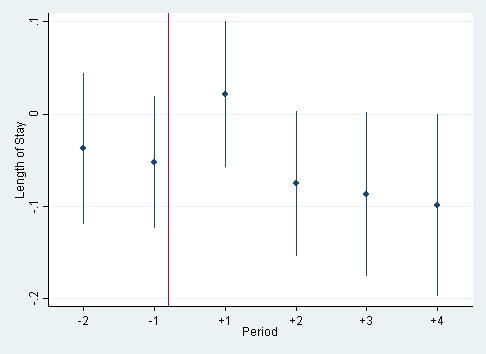
\includegraphics[height=2.5in,width=5in,keepaspectratio]{EventLOS_2011}
    \end{figure}
\end{frame}


\begin{frame}{Differential Trends}
    \begin{table}[htb!]
    \centering
    \footnotesize
    \centerline{
    \begin{tabular}{l|rrr}
        & Vert. Int.      & Practice Size & Beds \\
        \hline
        \multicolumn{3}{l}{$\Gamma_{jkt}$} \\
        \hline
        Charge          &     258.516    &      20.670*** &     192.032**  \\
                        &   (191.137)    &     (3.676)    &    (86.632)    \\
        LOS             &       0.005    &       0.002*** &       0.012    \\
                        &     (0.018)    &     (0.000)    &     (0.008)    \onslide<2->{\\
        \hline
        \multicolumn{3}{l}{$\Gamma_{jkt}$ with quality} \\
        \hline
        Charge          &     241.378    &      20.390*** &     188.895**  \\
                        &   (190.720)    &     (3.666)    &    (86.373)    \\
        LOS             &       0.003    &       0.002*** &       0.011    \\
                        &     (0.018)    &     (0.000)    &     (0.008)   }\\
    \end{tabular}}
    \end{table}

\end{frame}


\begin{frame}{Endogeneity of physician-hospital integration}
    \only<1>{
        Integration could be driven by:
        \begin{itemize}
            \item Existing physician behaviors
            \item Unobserved, time-varying practice characteristics
        \end{itemize}
    }
    \only<2>{
        \metroset{block=fill}
        \begin{block}{1. Set of possible physician-hospital pairs}
            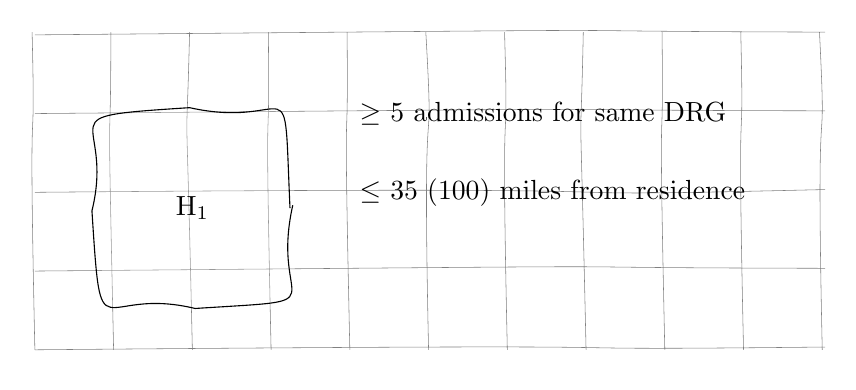
\begin{tikzpicture}[decoration=penciline, decorate]
                \draw[decorate,style=help lines] (0,0) grid[step=1cm] (10,4);

                % Patient 1
                \node[decorate,draw,inner sep=.7cm,fill=white,fill opacity=.2,text opacity=1,circle] (a) at (2,1.8) {$\text{H}_{1}$};

                \node[right] at (4,3) {$\geq$ 5 admissions for same DRG};
                \node[right] at (4,2) {$\leq$ 35 (100) miles from residence};
            \end{tikzpicture}
        \end{block}
    }
    \only<3>{
        \metroset{block=fill}
        \begin{block}{1. Set of possible physician-hospital pairs}
            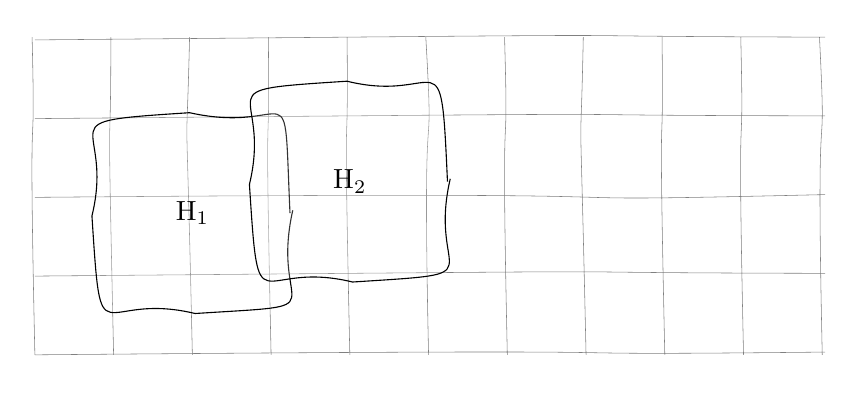
\begin{tikzpicture}[decoration=penciline, decorate]
                \draw[decorate,style=help lines] (0,0) grid[step=1cm] (10,4);

                % Patient 1
                \node[decorate,draw,inner sep=.7cm,fill=white,fill opacity=.2,text opacity=1,circle] (a) at (2,1.8) {$\text{H}_{1}$};

                % Patient 2
                \node[decorate,draw,inner sep=.7cm,fill=white,fill opacity=.2,text opacity=1,circle] (a) at (4,2.2) {$\text{H}_{2}$};

            \end{tikzpicture}
        \end{block}
    }
    \only<4>{
        \metroset{block=fill}
        \begin{block}{1. Set of possible physician-hospital pairs}
            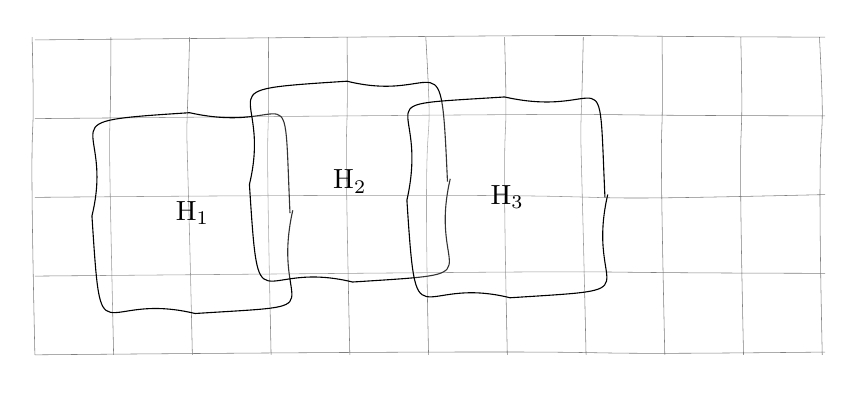
\begin{tikzpicture}[decoration=penciline, decorate]
                \draw[decorate,style=help lines] (0,0) grid[step=1cm] (10,4);

                % Patient 1
                \node[decorate,draw,inner sep=.7cm,fill=white,fill opacity=.2,text opacity=1,circle] (a) at (2,1.8) {$\text{H}_{1}$};

                % Patient 2
                \node[decorate,draw,inner sep=.7cm,fill=white,fill opacity=.2,text opacity=1,circle] (a) at (4,2.2) {$\text{H}_{2}$};

                % Patient 3
                \node[decorate,draw,inner sep=.7cm,fill=white,fill opacity=.2,text opacity=1,circle] (a) at (6,2) {$\text{H}_{3}$};

            \end{tikzpicture}
        \end{block}
    }
    \only<5>{
        \metroset{block=fill}
        \begin{block}{1. Set of possible physician-hospital pairs}
            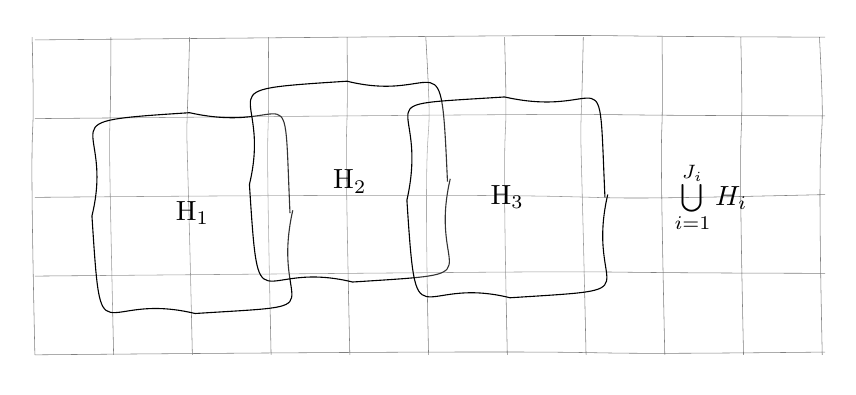
\begin{tikzpicture}[decoration=penciline, decorate]
                \draw[decorate,style=help lines] (0,0) grid[step=1cm] (10,4);

                % Patient 1
                \node[decorate,draw,inner sep=.7cm,fill=white,fill opacity=.2,text opacity=1,circle] (a) at (2,1.8) {$\text{H}_{1}$};

                % Patient 2
                \node[decorate,draw,inner sep=.7cm,fill=white,fill opacity=.2,text opacity=1,circle] (a) at (4,2.2) {$\text{H}_{2}$};

                % Patient 3
                \node[decorate,draw,inner sep=.7cm,fill=white,fill opacity=.2,text opacity=1,circle] (a) at (6,2) {$\text{H}_{3}$};

                \node[right] at (8,2) {$\bigcup\limits_{i=1}^{J_{i}} H_{i}$};
            \end{tikzpicture}
        \end{block}
    }
    \only<6>{
        \metroset{block=fill}
        \begin{block}{2. Estimate probability of integration (at practice level)}
            \begin{equation*}
                I_{pk} = \lambda z_{pk} + \omega_{pk}
            \end{equation*}
            \vspace{-.3in}
            \begin{itemize}
                \item Average choice set size
                \item Average differential distance (relative to nearest hospital)
                \item Differential distance interacted with hospital characteristics
            \end{itemize}
        \end{block}
    }
    \only<7>{
        \metroset{block=fill}
        \begin{block}{2. Estimate probability of integration}
            \begin{equation*}
                I_{pk} = \lambda z_{pk} + \omega_{pk}
            \end{equation*}
            \vspace{-.3in}
            \begin{itemize}
                \item Average choice set size
                \item Average differential distance (relative to nearest hospital)
                \item Differential distance interacted with hospital characteristics
            \end{itemize}
        \end{block}
        \begin{equation*}
            \hat{\Gamma}_{jkt} = \gamma_{j} + \gamma_{k} + \tau_{t} + \underbrace{I_{jkt}}_{\mathclap{\hat{I}_{jkt}=\text{Pr}(I_{jkt}=1)}} \delta_{1}  + \tilde{z}_{jkt}\delta_{2} + \eta_{jkt},
        \end{equation*}
    }
\end{frame}


\begin{frame}{Summary of Preliminary Results}
    \only<1>{
        \metroset{block=fill}
        \begin{block}{Effects of Vertical Integration}
            \begin{itemize}
                \item Increase in shares of about 7 percentage points (10\%)
                \item No improvement in mortality
                \item Potential increase in charges but relatively small (no more than 1.5\% or \$850 per operation)
            \end{itemize}
        \end{block}
    }

    \only<2>{
        \metroset{block=fill}
        \begin{block}{Effects of Practice Size}
            10-person increase in practice, \$200-\$250 increase in charge
        \end{block}
    }

    \only<3>{
        \metroset{block=fill}
        \begin{block}{Effects of Bed Size}
            Increase of 100 beds, \$150-\$200 increase in charge
        \end{block}
    }

\end{frame}

\begin{frame}{Next Steps}
    \begin{itemize}
        \item Exclude never-integrating hospitals    
        \item Identify physician ``movers''
        \item Focus on specific DRG (470)
        \item Examine institutional care beyond the inpatient stay
    \end{itemize}
\end{frame}

\end{document}






